%Roman Urdu:
%Unique words: 42 927
%Total words: 92 762 207
%Lines: 6 365 808

%Urdu
%Unique words: 43 783
%Total words: 92 849 342
%Lines: 6 365 808

\RequirePackage[no-math]{fontspec}
\documentclass[format=acmsmall,review=true,screen=true]{acmart}

%You can use any of these two fonts...
\newfontfamily\urdufont{Noto Naskh Arabic}[Script=Arabic,Language=Urdu]
%\newfontfamily\urdufont[Script=Arabic,Scale=1,Language=Urdu]{Jameel Noori Nastaleeq Kasheeda.ttf}
\ifxetex
\TeXXeTstate=1
\DeclareTextFontCommand{\texturdu}{\beginR\urdufont\aftergroup\endR}
\fi
\ifluatex
\DeclareTextFontCommand{\texturdu}{\textdir TRT\urdufont}
\fi
\usepackage{graphicx,subfigure}
\usepackage{hyperref}
\usepackage[autostyle]{csquotes}
\begin{document}

    \title{Urdu and Roman-Urdu Word Embeddings}
    
    \section{Introduction}
Word embeddings (also called vector representations or distributed representations) are high dimensional vectors consisting of real numbers which capture the syntactic and semantic meanings of the words. Closely related words are mapped near each other in a n-dimensional vector space. In other words, the cosine similarity of these vectors is close to 1. These representations aid in various natural language processing tasks like sentiment analysis, text summarization, named entity recognition etc.\\

    \section{Literature Survey}
    
    Word embeddings have been used in a wide array of applications such as text classification, sentiment analysis and ontology enrichment \cite{RaoS16,sentanalysis,Pembeci2016UsingWE}. Word embeddings have also been applied to Automatic Query Expansion \cite{RoyPMG16}, Biomedical Named Entity Recognition task \cite{chang2015application} and image captioning \cite{10.1145/2964284.2964299}. Word embeddings have also been of use in solving problems across different languages such as Bengali \cite{ahmad2016bengali} and Arabic \cite{7841054}.\\\\
    The word embeddings obtained by these techniques have many applications. A paper \cite{tshitoyan2019unsupervised} describes how training a model on material science literature is able to capture concepts like the structure-property relationships in materials. It can also suggest materials for applications well before their discovery. In another paper \cite{gligorijevic2016large} demonstrates that the embeddings obtained from a large EHR database have yielded many improvements on disease phenotyping compared to traditional approaches. The embeddings also aided in discovering new disease-gene association. This proved that such techniques can help in minimizing costs of lab studies.Another significant application of word embeddings are recommendation systems. Many large companies use them to offer suggestions to users. For example, \cite{grbovic2018real} explains how Airbnb used Word2Vec to enhance its recommendations, which helped improve its revenue stream.\\\\
    Word2Vec \cite{mikolov2013distributed} was developed by Tomas Mikolov at Google in 2013 and is one of the most popular techniques to learn word embeddings. It used local context around a word to learn embeddings and contains two variants: Skip-gram and Continuous Bag Of Words. GloVe \cite{pennington2014glove} was later introduced by Stanford which used local statistics as well as global statistics by using a global word co-occurrence matrix to generate embeddings. fastText \cite{arm2016bag} was developed and introduced by Facebook in 2015 for efficient learning of word representations. Apart from the word itself, each word in fastTest is represented as a bag of character n-grams which helps preserve meaning of short words and also helps fastText tackle rare words. fastText has also helped reduce training and testing time complexities for classifiers from linear to logarithmic by making use of a hierarchical classifier based on a Huffman coding tree.\\\\
    ELMo \cite{peters2018deep} and BERT \cite{devlin2018bert} are two recent additions to the NLP world that achieved state of the art results over a number of NLP tasks. ELMo was developed in 2018 by AllenNLP and BERT later that year by Google’s Research Group. Both differ from static models such as Word2Vec , GloVe  and fastText as the embeddings they produce are contextual in nature. Unlike static models that assign a fixed embedding to a word, irrespective of the different contexts in which it may have occurred, contextual models determine embeddings based on context, hence a single word can have more than one embedding assigned to it. \\\\
    There is some work done with word embeddings in the Urdu language. \cite{haider2018urdu} trained the skip-gram variant of Word2Vec with different parameters and evaluated the models over a word similarity task. \cite{alam2017sequence} used Word2Vec embeddings for a Roman-Urdu to Urdu transliteration system. \cite{pourdamghani2018using} describes how Word2Vec's embeddings were used to improve word alignments to translate 15 low resource languages (including Urdu) into English. The results exhibited improving BLEU scores. In \cite{bhat2016house}, Word2Vec was used to bridge the differences between Hindi and Urdu languages. In \cite{shahid2019rewriter}, word embeddings were used to design a model for text summarization. \cite{khan2019deep} describes how word embeddings were used to enhance Named Entity Recognition approaches for the Urdu language. \\\\
    Not much work has been done with regards to word-embeddings in Roman Urdu. \cite{memood2020precisely} used neural word embeddings from models such as Word2Vec, fastText and GloVe in Roman Urdu Sentiment Analysis and evaluated these models over metrics such as accuracy, precision, recall and F1 score. \cite{khan2020clustering} used Word2Vec clustering in their experiments for lexical normalization of Roman Urdu corpora. 
    \subsection{Research Gap} 
    Following the release of word2vec by Google in 2013, a lot of work has been done in the domain of word embeddings. Many more methods have been released which use different techniques to obtain these distributed representations. word2vec and some of its extensions like GloVe, fastText, doc2vec and topic2vec generate context independent embeddings (i.e. a single embedding irrespective of how many different contexts a word may be used in). Others such as BERT and ELMo can be used to obtain context dependent embeddings. These models have been trained on a number of high-resource languages like English, Spanish and French. Various state-of-the-art benchmarks have been used to evaluate the models through tasks like analogy, similarity and categorization.\\
    
Although the amount of work being done in this domain is quite extensive, one area that remains neglected is work on low-resource languages like Urdu and Roman Urdu. Due to a lack of extensive, publicly available corpora, performing such work on these languages becomes very difficult. As we conducted our literature survey on this domain, we found no work done for Roman Urdu, whereas just a single paper was published for Urdu by Samar Haider \cite{haider2018urdu}. In this paper, he trained the Skip-Gram variant of the word2vec model on corpora totalling 140M+ words. He experimented with two of the parameters - context window size and vector dimensionality. To evaluate the performance of his models, he used the WordSim-353 \cite{} and SimLex-999 \cite{hill2014simlex999} datasets. These datasets consist of word pairs which have been manually assigned a score based on how related or similar they are. To compare the predictions of his models, he used Spearman’s Correlation coefficient.However, Haider’s work was limited to just the Skip-Gram variant of word2vec. No work has been performed on any other variant or word-embedding technique for Urdu and Roman Urdu in particular. This is the research gap that we aim to close with this project. We plan to train models for both Urdu and Roman Urdu languages and the methods we will be using include word2vec (both CBOW and Skip-Gram variants), GloVe, fastText, ELMo and BERT. We will then perform a comparative analysis of these models and observe their performance on these languages. We hope that our work will pave the way for further work to be done in the field of Natural Language Processing on Urdu and Roman Urdu languages.

    \section{Models' Architecture Details}
    \subsection{Word2Vec}
    Word2Vec \cite{mikolov2013distributed} introduced two new model architectures that aimed to reduce computational complexity which was caused by the non-linear hidden layer in the Neural Network Language Models. It consists of two models: Continuous Bag of Words and Skip-gram. In CBOW, the non-linear hidden layer is removed and the projection layer is shared for all words, which means all words are projected onto the same position. A log-linear classifier is used with a certain number of words before and after the target word which are used as the context to print the target word. In other words, the current word is predicted based on the context. Skip-gram on the other hand works by maximizing classification of a word based on another word in the same sentence. More specifically, the current word is used as an input to a log-linear classifier with a continuous projection layer to predict words within a certain range before and after the current word. In other words, the current word is used to predict the context.
    \subsection{Glove}
    GloVe \cite{pennington2014glove}, developed by Stanford, is a log-bilinear model that uses both global matrix factorization and local context window methods to create embeddings. It generates a word-word co-occurrence matrix over the corpus which stores counts of words occurring with each other within a given context window. Matrix factorization techniques are then applied on the matrix for dimension reduction. It trains a weighted least squares model on this matrix. The objective here is to learn vectors such that their dot product is the same as the logarithm of the words' probability of co-occurrence.
    
    The model uses ratios of the co-occurrence probabilities rather than the raw co-occurrence probabilities as the starting point for vector learning. To handle co-occurrences that occur rarely, a weighted least squares regression model is used. This model generates two different vectors for each word. If the co-occurrence matrix is symmetric, the difference in the vectors is caused by their random initialization.
    \subsection{FastText}
    fastText \cite{arm2016bag} is a modified linear classifier which can work with a large dataset. It employs a rank constraint on the classifier, and uses a softmax function to calculate probability distributions. This hierarchical softmax, based on Huffman coding tree, helps reduce the running time from O(kh) to O(h log2 k). It further improves its efficiency by using a depth-first search algorithm, which discards small probability branches.
    
    In addition to the word embeddings, fastText also uses a bag of n-grams to represent a word. For example, considering the word “machine”, with n = 3, the model would represent this word as <ma, mac, ach, chi, hin, ine, in>, where the angular brackets denote the start and the end of the word. This allows fastText to extract much more information from words than other models. 
    \subsection{BERT}
    BERT differs from previous techniques by incorporating a transformer architecture that consists of multiple encoder layer stacked upon one another. It has two variants, namely: \texorpdfstring{BERT\textsubscript{base}}{} and \texorpdfstring{BERT\textsubscript{large}}{}. The base model has 12 encoder layers, 768 Feed Forward Networks, 12 Attention Heads and a total of 110M parameters whereas the large model has 24 encoder layers, 1024 Feed Forward Networks, 16 Attention Heads and a total of 340M parameters.\\
    
BERT can be pretrained on a large un-labelled text corpus and can later be finetuned to any task specific dataset. Pre-training comprises of two key phases: Masked Language Modelling (MLM) and Next Sentence Prediction (NSP). In MLM 15\% of token positions in the sentences passed are chosen at random and masked and the surrounding words are used to predict the masked token. BERT expects pairs of sentences concatenated together as input with a separation token between them. In NSP, sentences A and B for each pair passed are selected in a randomized manner from the corpus such that 50\% of the time B is the actual sentence that follows A and 50\% of the time B it is not. The model predicts whether or not sentence B follows A or not. Once the model has been pretrained it can later be finetuned to support a variety of different NLP tasks through minor modifications to the output of the model.


    \subsection{ELMo}
    ELMo runs multi-layer forward and backward LSTMs to compute the embeddings. It starts by first assigning a character level embedding to the tokens that are passed. Character level embeddings aid in capturing morphological features of the tokens that are passed to them. These embeddings are passed through a series of layers before being forwarded to a 2-layer high-way network. The biLM model has two layers stacked together where each layer has two passes - forward pass and backward pass. The forward pass contains information about a certain word and captures the context before that word. In the backward pass, the information about the word is captured along with the context after that word. This pair of information forms the intermediate word vectors.  ELMo calculates the weighted sum of the raw word vectors and the intermediate word vectors. This allows for semi-supervised learning, where the biLM is pre-trained at a large scale and easily incorporated into other neural architectures.
    \section{Results and Analysis}

    
    
    \subsection{Quantitative Analysis}
    To perform quantitative analysis, we used SimLex-999 and WordSim-353 datasets. SimLex-999 contains 999 word pairs and are used to observe how well our models capture similarity between words. WordSim-353 contains 353 word pairs which is used to measure how well it captures similarity as well as relatedness between words. Both of these datasets contain scores which are assigned by the annotators and agreed upon, that rate how similar or related the word pairs are. The following figures show what these datasets look like:
    
    \begin{left}
    \begin{tabular}{ |c|c|c| } 
    \hline
    Word A & Word B & Score \\
    \hline
    kitaab & kaghaz & 7.46 \\ 
    computer & internet & 7.58 \\
    train & car & 6.31 \\
    \hline
    \end{tabular}
    \end{left}
    
    \begin{right}
    \begin{tabular}{ |c|c|c| } 
    \hline
    Word A & Word B & Score \\
    \hline
    کتاب &کاغذ & 7.46 \\ 
    computer & internet & 7.58 \\
    train & car & 6.31 \\
    \hline
    \end{tabular}
    \end{right}
    
    
    Since we are conducting our research in the Urdu and Roman Urdu languages, we had to translate the SimLex and WordSim datasets to Urdu and then transliterate to Roman Urdu. We translated the word pairs from English to Urdu using Google’s translate service. Certain words which Google Translate failed to translate or showed irregular translations, such as single words being translated into phrases, were removed from the dataset. Words from Urdu were then transliterated to Roman Urdu using iJunoon’s Urdu to Roman Urdu transliteration service.
    
    For evaluating our models on these datasets, we used Spearman’s Rank Correlation which is a technique used to calculate the strength and direction between two variables. It returns a value from -1 to 1 where:

    +1:	a perfect positive correlation between variables
    
    -1:	a perfect negative correlation between variables
    
    0: no correlation between variables
     
    The Spearman’s Rank Correlation is represented by the formula:
    \begin{equation*}
    \rho = 1-\frac{6\sum d^2_i}{n(n^2 - 1)}
    \end{equation*}
    where,
    
    n is the number of observations,
    
    $ d_i $ is the difference in rank between the $ i^{th} $ observations
    
    \begin{table}[]
    \begin{tabular}{|l|l|l|}
    \hline
                           & \textbf{WordSim-353} & \textbf{SimLex-999}    \\
    \hline
    \textbf{Word2Vec CBOW} &         0.495             &      0.189                  \\
    \hline
    \textbf{Word2Vec SG}   &    0.485                  &    0.186                   \\
    \hline
    \textbf{fastText CBOW} &        0.406              &         0.165              \\
    \hline
    \textbf{fastText SG} &          0.474            &      0.199                  \\
    \hline
    \textbf{GloVe} &        0.367              &        0.095                \\
    \hline
    \textbf{ELMo} &         -0.067             &        0.097               \\
    \hline
    \textbf{BERT} &         0.327             &         0.123            \\
    \hline
    \end{tabular}
    \end{table}
    
    \begin{table}[]
    \begin{tabular}{|l|l|l|}
    \hline
                           & \textbf{WordSim-353} & \textbf{SimLex-999}    \\
    \hline
    \textbf{Word2Vec CBOW} &         0.517             &      0.165                  \\
    \hline
    \textbf{Word2Vec SG}   &    0.527                  &    0.205                   \\
    \hline
    \textbf{fastText CBOW} &        0.465              &         0.122              \\
    \hline
    \textbf{fastText SG} &          0.544            &      0.144                  \\
    \hline
    \textbf{GloVe} &        0.442              &        0.137                \\
    \hline
    \textbf{ELMo} &         0.156             &        0.079               \\
    \hline
    \textbf{BERT} &         0.039             &         -0.083            \\
    \hline
    \end{tabular}
    \end{table}
    
    If we compare our Urdu scores with those of \cite{haider2018urdu}, we can observe that they are quite close to his own score. Whereas \cite{haider2018urdu} used different embedding sizes of 100, 200 and 300, we used an embedding size of 500. \cite{haider2018urdu} also varied the size of the context window and chose them to be 3, 5 and 7 while we fixed ours to be 5. \cite{haider2018urdu} trained only a single model which was the Word2Vec Skip-gram model while we trained both the CBOW and Skip-gram variants of Word2Vec and on top of that trained models for fastText and GloVe as well. For the WordSim-353 dataset, the best score \cite{haider2018urdu} was able to get was 0.524 on a context window size of 5 and dimensionality 200 while we were able to achieve 0.485. For the SimLex-999 dataset, \cite{haider2018urdu} was able to get a best score of 0.306 on a context window size of 7 and dimensionality 300 while we got a score of 0.186. The lower score could be explained by the fact that SimLex-999 is a challenging dataset with a high variety of words. Static models such as word2vec, fastText and GloVe gave comparable results however the embeddings extracted from the contextual models such as BERT and ELMo did not score that high. This verifies the fact that raw embeddings from these models aren’t as useful. These models need to be fine-tuned with task-specific datasets to yield better results. The embeddings produced by these models are not fixed and change according to context.

    
    \subsection{Qualitative Analysis}
To perform a qualitative analysis of the embeddings generated by the models, we essentially generated plots of two types - word-word and word-cluster. These plots show how the models project related words in a vector space. To generate these plots, we used matplotlib to create scatter plots.
Since we trained the models to generate high dimensional (500) embeddings, the first thing we needed to do was transform the vectors to lower dimensions (in this case, 2). To achieve this, we used the scikit-learn library.\\

\textbf{1. Word-Word Plots}\\
We chose word pairs spanning various categories, like country-capital, word-synonym, word-antonym and singular-plural. The words chosen from these categories were carefully selected, in order to display meaningful plots to the viewer.\\

To perform dimensionality reduction for our word-word plots, we used Principal Component Analysis from the scikit-learn library. This performs linear dimensionality reduction using Singular Value Decomposition of an embedding to project it to a lower dimension. To connect the word-word pairs, we drew line segments between the plotted embeddings.\\

\textbf{1.1 Urdu}\\

For the plots generated for the country-capital pairs, the key thing to observe was the direction in which a country was plotted relative to its capital. The SG variant of Word2Vec does not yield consistent directions for any of the word pairs. The CBOW variant on the other hand gives the same direction for the pairs except \texturdu{افغانستان  کابل}. GloVe’s plot shows the pairs have two different directions. For the SG variant of fastText, the \texturdu{عراق  بغداد} pair is an outlier. The CBOW variant, unlike that of Word2Vec, does not exhibit the same consistency. The plot given by ELMo’s embeddings shows two different directions for two pairs of the country-capital pairs. Meanwhile, for BERT, the \texturdu{ ٹوکیو جاپان} pair is a clear outlier.
For the word-synonym pairs, the main property to observe is the distance between the embeddings. The SG variant of Word2Vec plots \texturdu{ ہنس  مسکرا} pair on the point while the others are at some distance. In the plot for the CBOW variant, the \texturdu{خوبصورت دلکش} pair is the closest. The GloVe model was unable to plot any of the pairs in close proximity. The \texturdu{ ہنس  مسکرا} pair is well placed in plot for the SG variant of fastText, while the \texturdu{ خوبصورت دلکش} pair is the best placed pair in the CBOW variant’s plot.\\

    \begin{table}[]
    \begin{tabular}{|l|l|}
        \hline
                            \textbf{Country} & \textbf{Capital}    \\
    \hline
    \texturdu{افغانستان}             &      \texturdu{کابل}\\
       \hline
    \hline
    \texturdu{جاپان}             &      \texturdu{ٹوکیو}\\
       \hline
    \hline
    \texturdu{انگلینڈ}             &      \texturdu{لنڈن}\\
       \hline
    \hline
    \texturdu{عراق}             &      \texturdu{بغداد}\\
       \hline
    \end{tabular}
                \caption{\label{tab:table-name}Urdu Country-Capital Pairs}
    \end{table}
    
        \begin{table}[]
    \begin{tabular}{|l|l|}
        \hline
                            \textbf{Word} & \textbf{Synonym}    \\
    \hline
    \texturdu{خدا}             &      \texturdu{پروردگار}\\
       \hline
    \hline
    \texturdu{خوبصورت}             &      \texturdu{دلکش}\\
       \hline
    \hline
    \texturdu{ہنس}             &      \texturdu{مسکرا}\\
       \hline

    \end{tabular}
            \caption{\label{tab:table-name}Urdu Word-Synonym Pairs}
    \end{table}

\textbf{1.2 Roman Urdu}\\

    \begin{table}[]
    \begin{tabular}{|l|l|}
        \hline
                            \textbf{Country} & \textbf{Capital}    \\
    \hline
    pakistan            &      islamabad\\
       \hline
    \hline
    japan             &      tokyo\\
       \hline
    \hline
    england             &      london\\
       \hline
    \hline
    iraq             &      bghdad\\
       \hline
    \end{tabular}
                    \caption{\label{tab:table-name}Roman Urdu Country-Capital Pairs}
    \end{table}
    
        \begin{table}[]
    \begin{tabular}{|l|l|}
        \hline
                            \textbf{Word} & \textbf{Synonym}    \\
    \hline
    khuda          &      parvardigaar\\
       \hline
    \hline
    khoobsurat            &      dilkash\\
       \hline
    \hline
    hans            &      muskura\\
       \hline

    \end{tabular}
        \caption{\label{tab:table-name}Roman Urdu Word-Synonym Pairs}
    \end{table}
We observed that generally the directions for the word pairs are consistent within a plot. This is true except for the iraq-bghdad pair plotted by both the variants of Word2Vec. The plots for the embeddings learned by GloVe also show the japan-tokyo and pakistan-islamabad pairs having different directions than the rest of the pairs. The SG variant of fastText shows different directions for almost every pair. The CBOW variant plots all but the iraq-bghdad pair in almost the same direction. The ELMo model’s plot only has the london-england and kabul-afghanistan pairs in the same direction. Meanwhile the plot from BERT’s embeddings was very inconsistent.\\

The SG variant of Word2Vec plots the hans-muskura pair in close proximity. In comparison, the CBOW variant plots. The plots showing GloVe’s representations of the word, only the dilkash-khoobsurat pair has a small distance. For the SG variant of fastText, the hans-muskura pair has the best learnt representation, as they have a very small distance in between. In the CBOW variant, the dilkash-khoobsurat pair is the best represented one.\\

\textbf{2. Word-Cluster Plots}\\
For cluster plots, we hand-picked a list of words and used clusters of words considered the closest to these by each of the models to make the scatter plots and see how close these related words are projected in a 2D vector space.\\

Here, dimensionality reduction is performed using t-distributed Stochastic Neighbor Embedding (TSNE) from scikit-learn. This changes similarities between the data points to joint probabilities and attempts to reduce the Kullback-Leibler divergence between the joint probabilities of the low dimensional representations and the high dimensional data.\\

\textbf{2.1 Urdu}\\

        \begin{table}[]
    \begin{tabular}{|l|l|}
        \hline
                            \textbf{No.} & \textbf{Word}    \\
    \hline
    1.            &      \texturdu{موسم}\\
       \hline
    \hline
    2.           &      \texturdu{کھانا}\\
       \hline
    \hline
    3.             &      \texturdu{مذہب}\\
       \hline
    \hline
    4.             &      \texturdu{صبح}\\
       \hline
        \hline
    5.             &      \texturdu{باپ}\\
       \hline
    \hline
    6.             &      \texturdu{حکومت}\\
       \hline
    \hline
    7.             &      \texturdu{امریکہ}\\
       \hline
    \hline
    8.             &      \texturdu{پاکستان}\\
       \hline
    \hline
    9.             &      \texturdu{مسلمان}\\
       \hline
    \hline
    10.             &      \texturdu{کرکٹ}\\
       \hline
    \hline
    11.             &      \texturdu{مذہب}\\
       \hline
    \hline
    12.             &      \texturdu{محمد}\\
       \hline      
    \hline
    13.             &      \texturdu{شہر}\\
       \hline     
    \hline
    14.             &      \texturdu{مالک}\\
       \hline     
    \hline
    15.             &      \texturdu{اللہ}\\
       \hline             
    \end{tabular}
        \caption{\label{tab:table-name}Urdu Words}
    \end{table}


The clusters plotted from the Word2Vec SG variant are not very useful. They are not as closely projected as they should be. The CBOW variant’s plot shows a very weird projection - two words, صلی and وسلم, are considered similar to some word but they are plotted quite far from the rest of the words. But the clusters again are not very meaningful. GloVe is able to project slightly better clusters, with some being closely projected. fastText’s plots are much better, with many clusters appropriately placed. The CBOW variant shows the best projections of the clusters. Neither ELMo nor BERT were able to give a meaningful cluster, although one thing to be noticed about ELMo’s clusters is that all the words have similar spellings. This can be attributed to the fact that ELMo is a character-based model.\\

\textbf{2.1 Roman Urdu}\\

        \begin{table}[]
    \begin{tabular}{|l|l|}
        \hline
                            \textbf{No.} & \textbf{Word}    \\
    \hline
    1.            &      mausam\\
       \hline
    \hline
    2.           &      khana\\
       \hline
    \hline
    3.             &      mazhab\\
       \hline
    \hline
    4.             &      subha\\
       \hline
        \hline
    5.             &      baap\\
       \hline
    \hline
    6.             &      hukoomat\\
       \hline
    \hline
    7.             &      america\\
       \hline
    \hline
    8.             &      pakistan\\
       \hline
    \hline
    9.             &      muslaman\\
       \hline
    \hline
    10.             &      cricket\\
       \hline
    \hline
    11.             &     mazhab\\
       \hline
    \hline
    12.             &      mohammad\\
       \hline      
    \hline
    13.             &      shehar\\
       \hline     
    \hline
    14.             &     maalik\\
       \hline     
    \hline
    15.             &      allah\\
       \hline           
       
    \end{tabular}
    \caption{\label{tab:table-name}Roman Urdu Words}
    \end{table}

The clusters plotted by the SG variant of Word2Vec are not very meaningful - for some of the clusters, the words are closely plotted, while for others are more spread-out. The CBOW variant does much better, with most of the similar words being in close proximity. GloVe’s representations roughly fall in between those of the Word2Vec variants. However, fastText’s clusters were the most interesting. Due to its capture of n-gram information, the clusters it makes consists of words which have similar spellings (or in other words, these words contain a substring of the main word). For example, the cluster for the word america contains words such as american, amreeci and ameriki. Among the two variants, the CBOW variant’s cluster was the most closely packed. And once again, we see that ELMo and BERT’s clusters are not meaningful, with the former’s clusters consisting of similarly spelt words.\\

Graphs Used are given below:\\

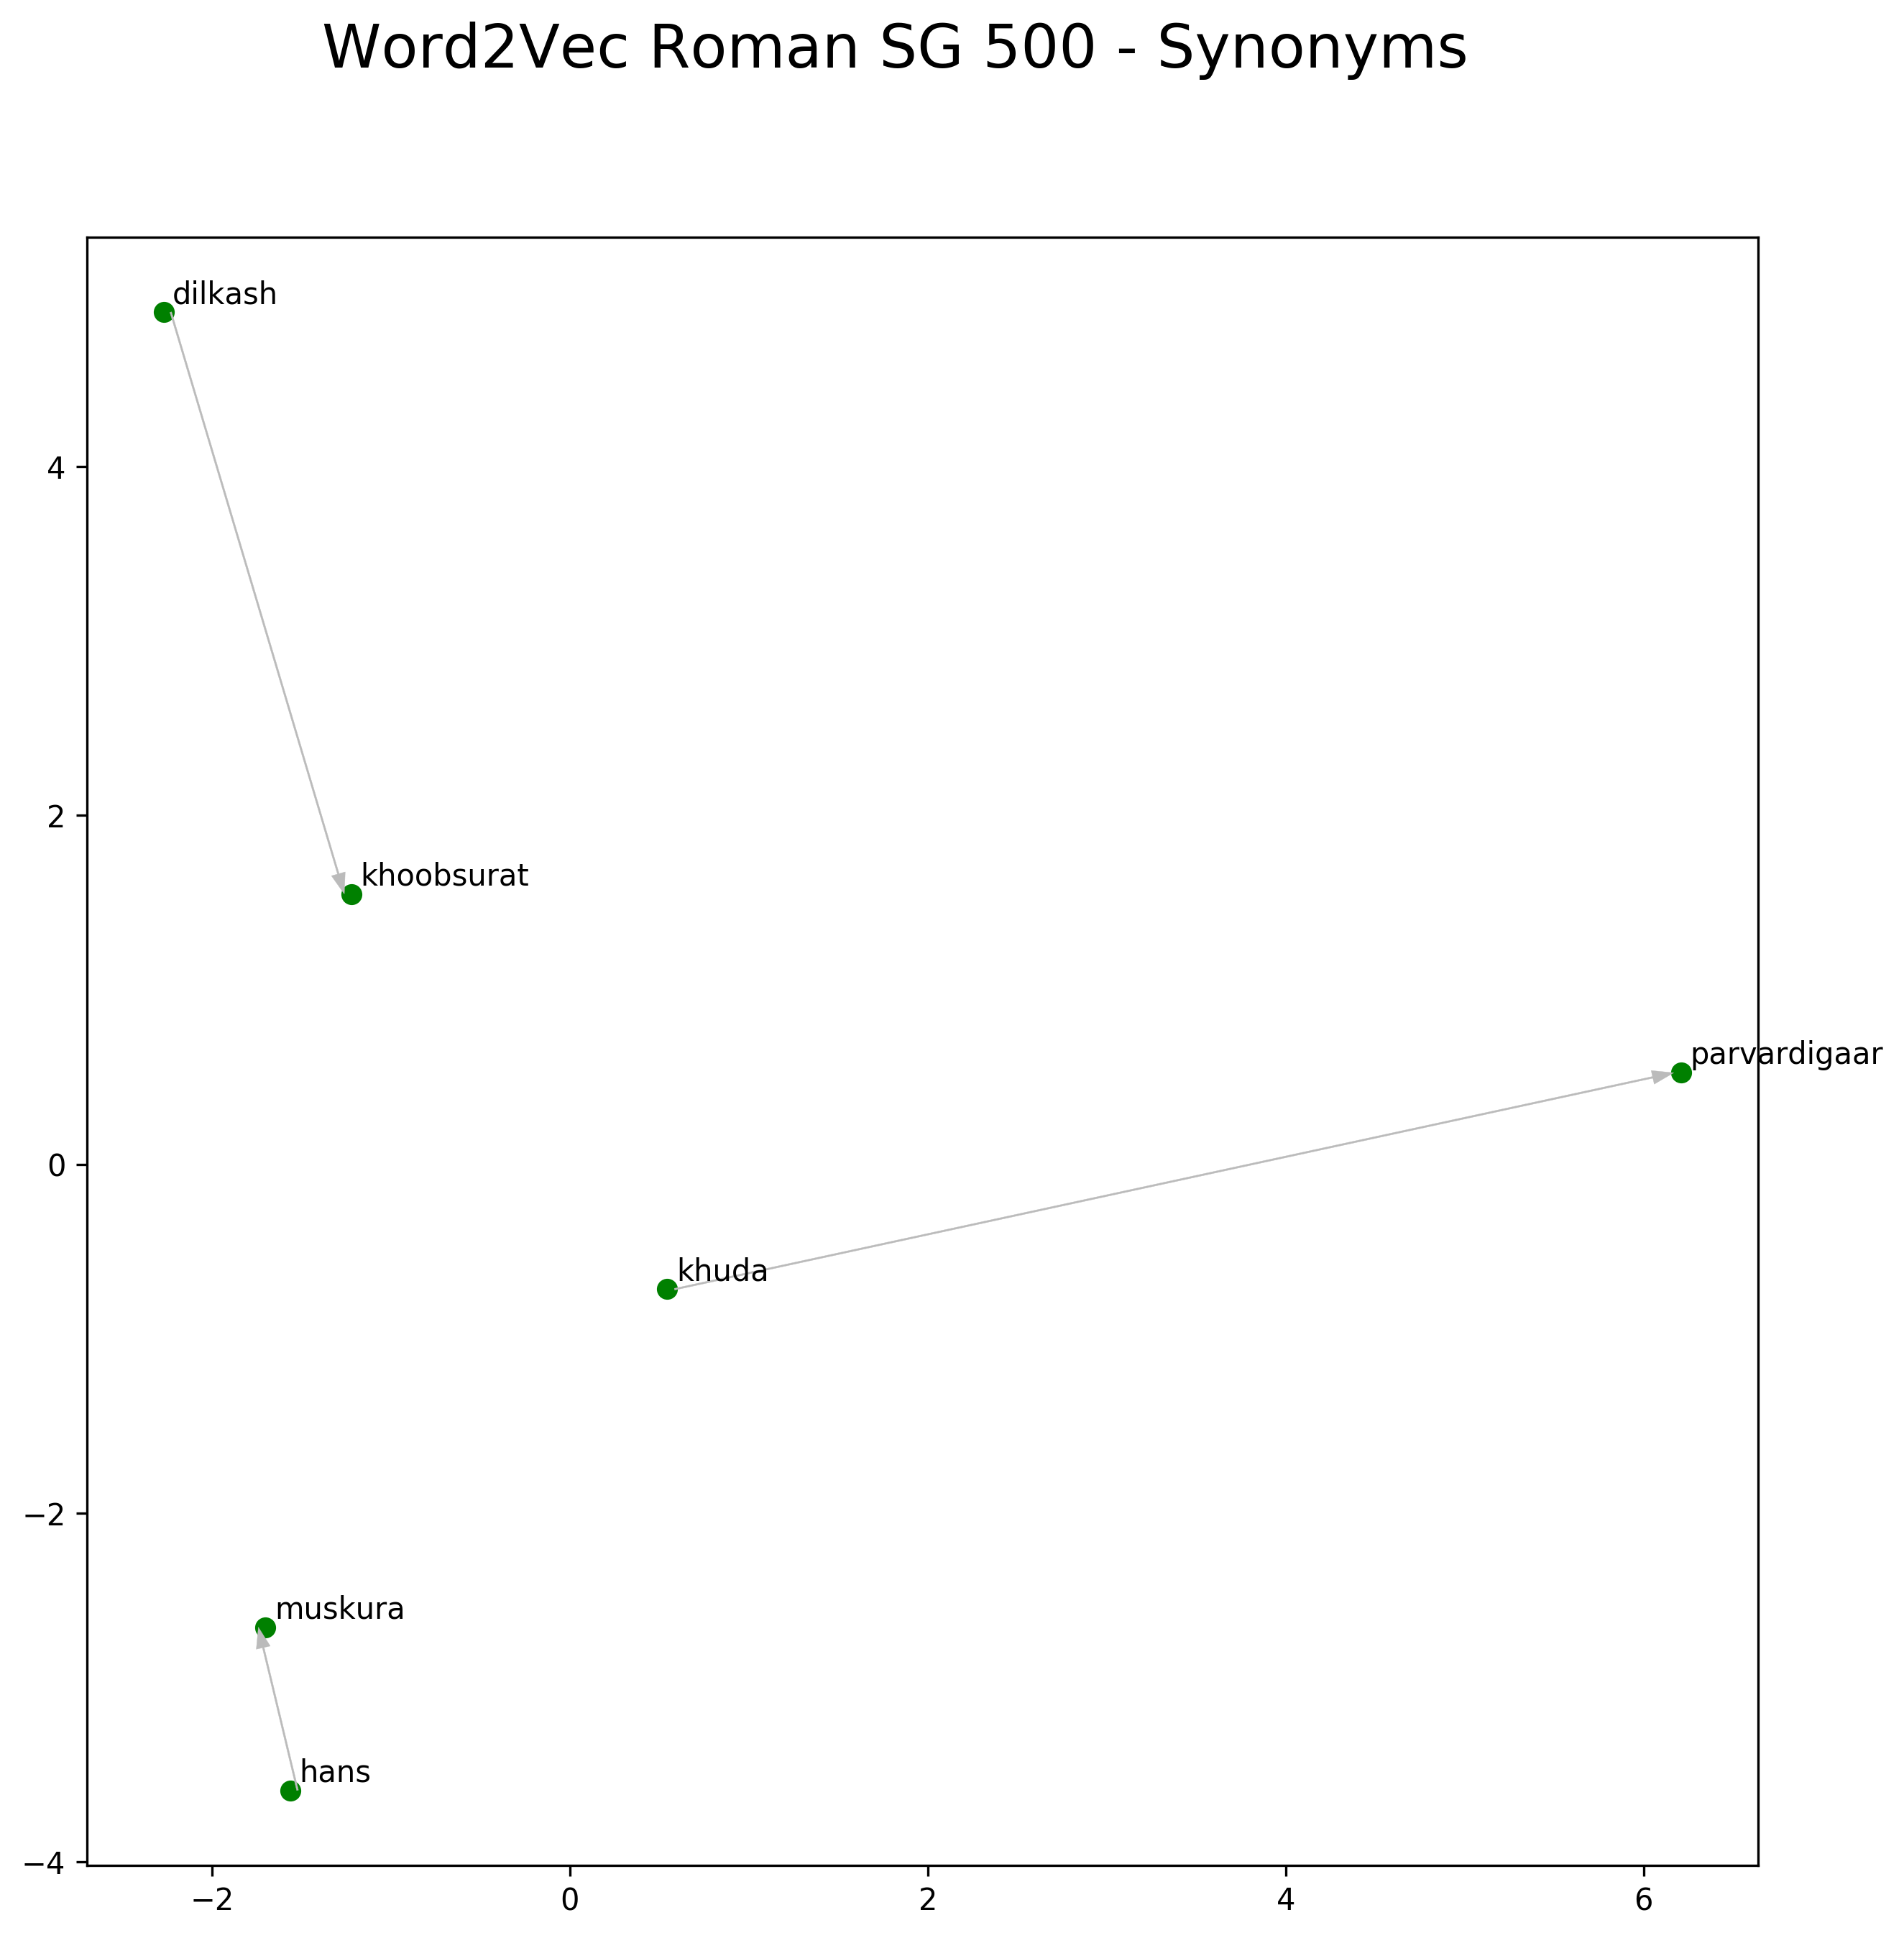
\includegraphics[width=10cm,height=10cm,keepaspectratio]{word2vec-sg_roman-urdu_synonyms.png}\\
\newpage
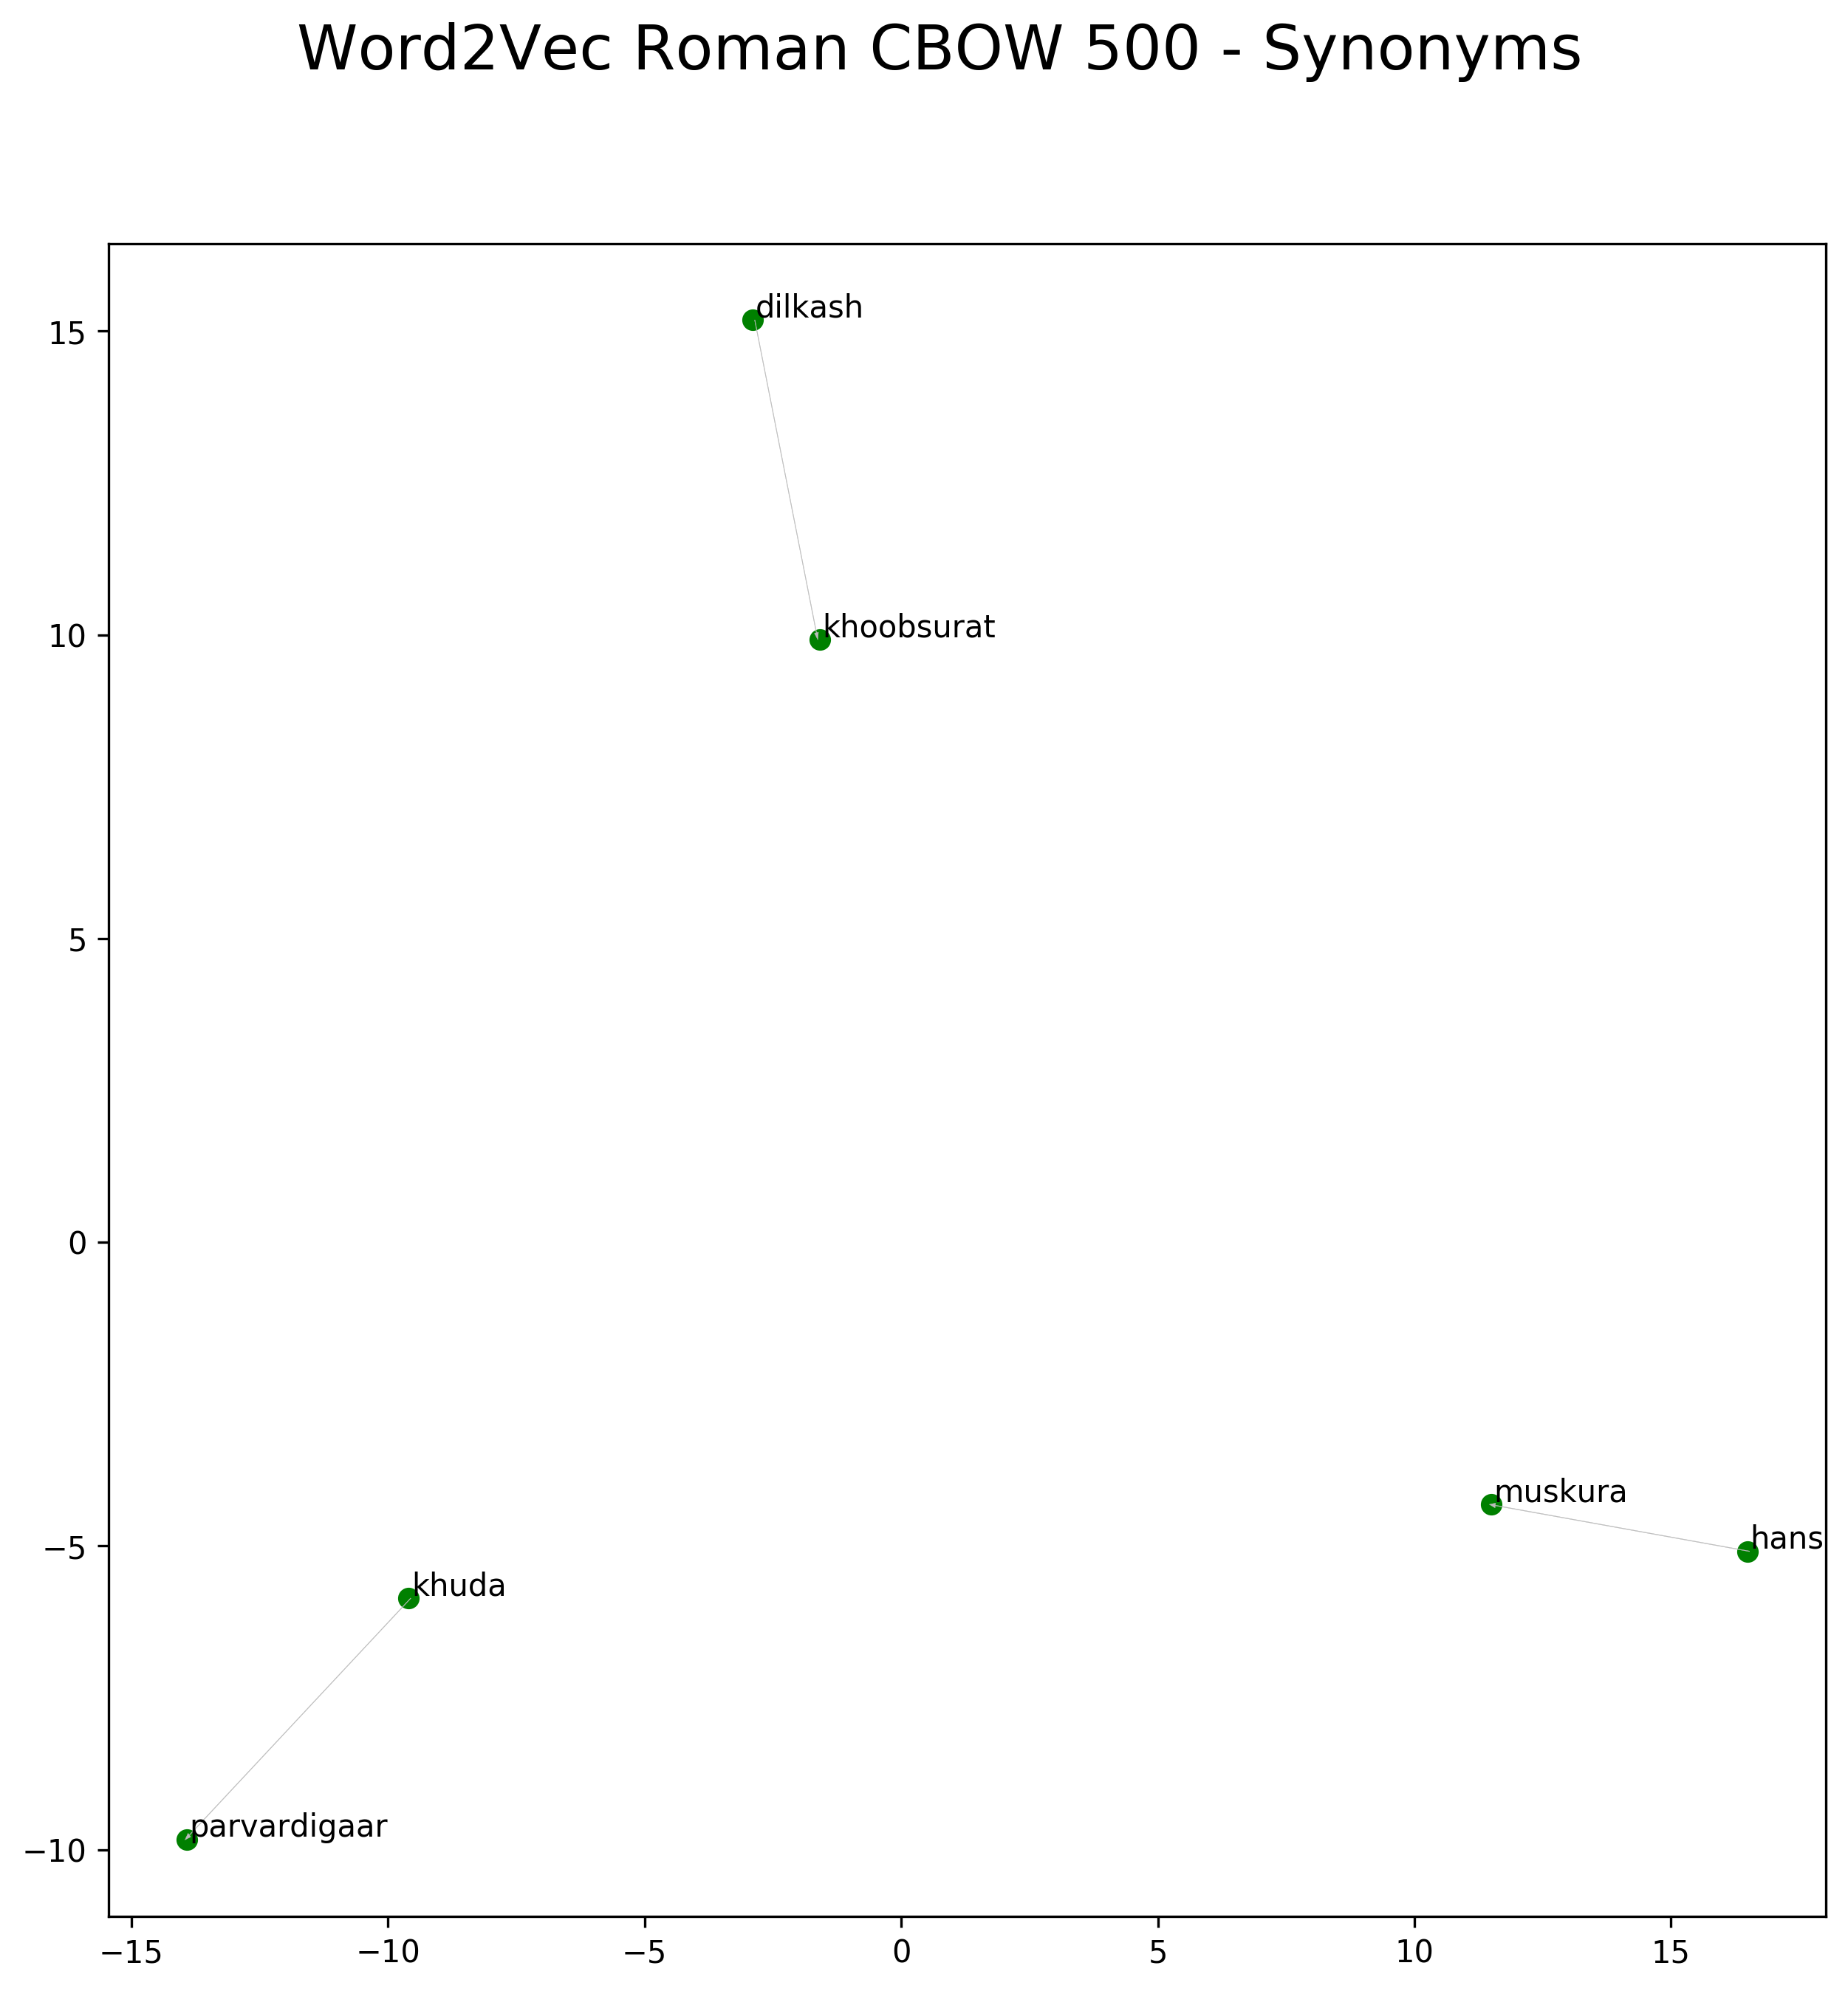
\includegraphics[width=10cm,height=10cm,keepaspectratio]{word2vec-cbow_roman-urdu_synonyms.png} \\
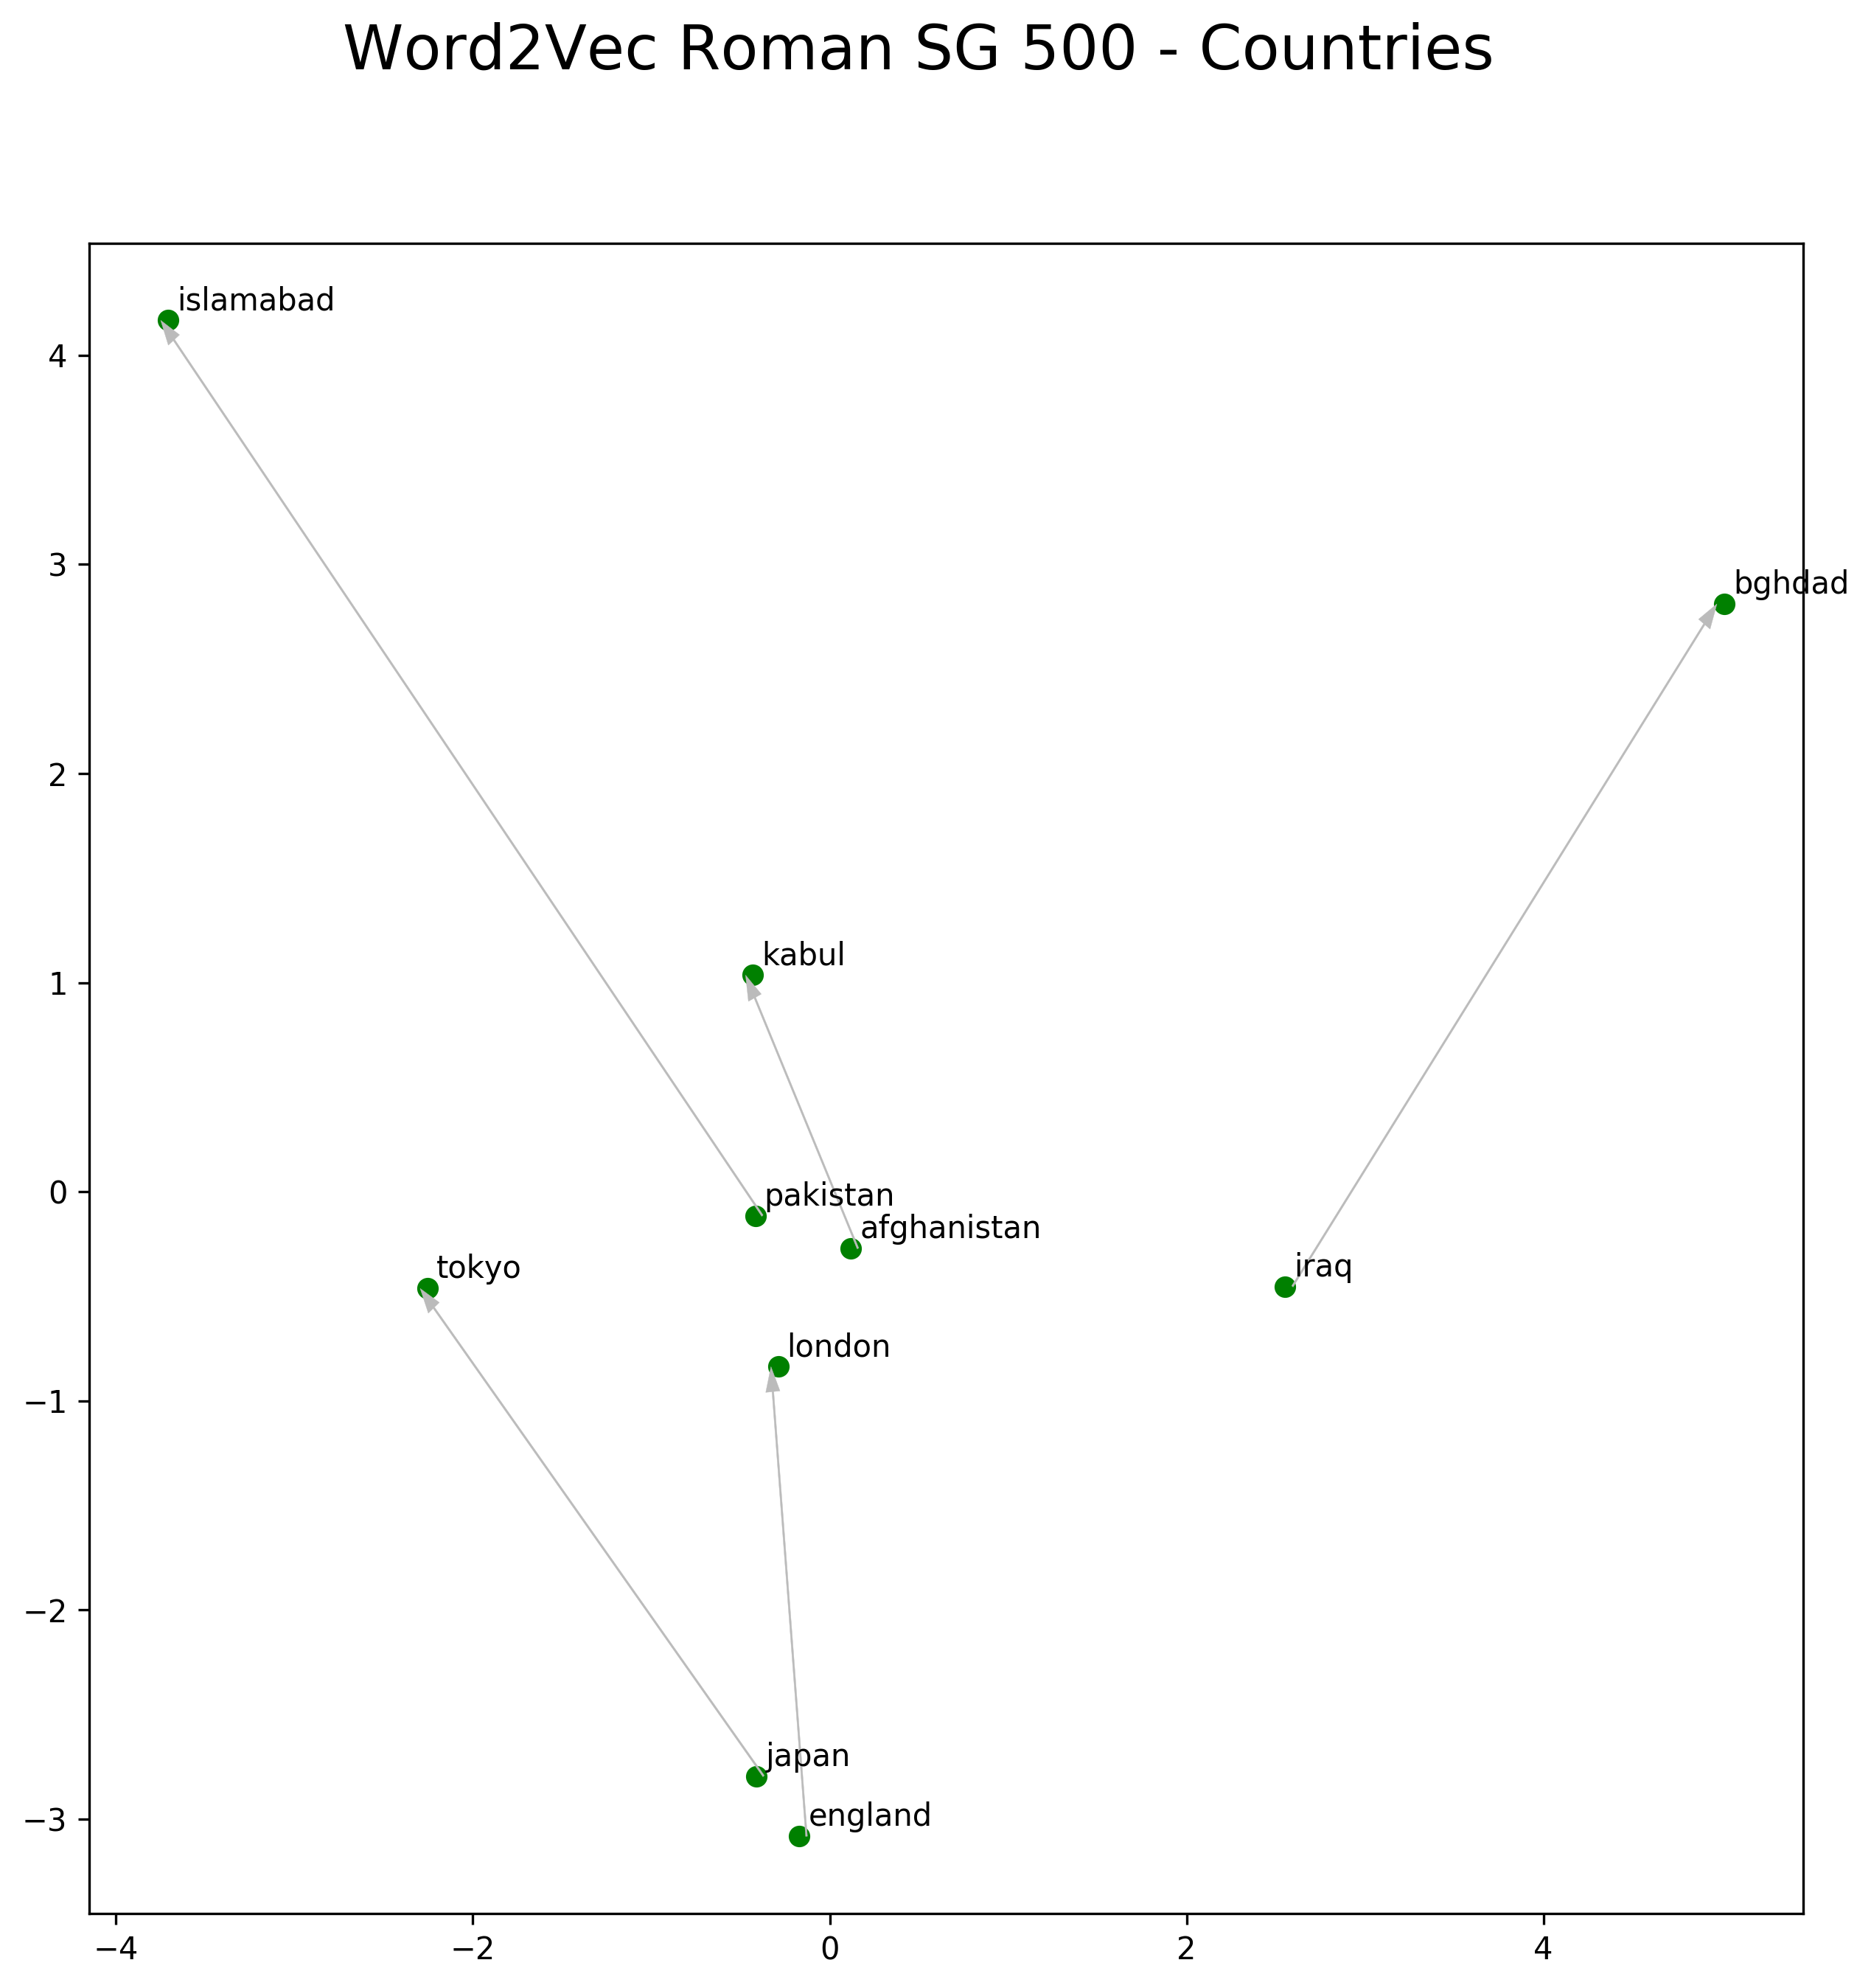
\includegraphics[width=10cm,height=10cm,keepaspectratio]{word2vec-sg_roman-urdu_countries.png} \\
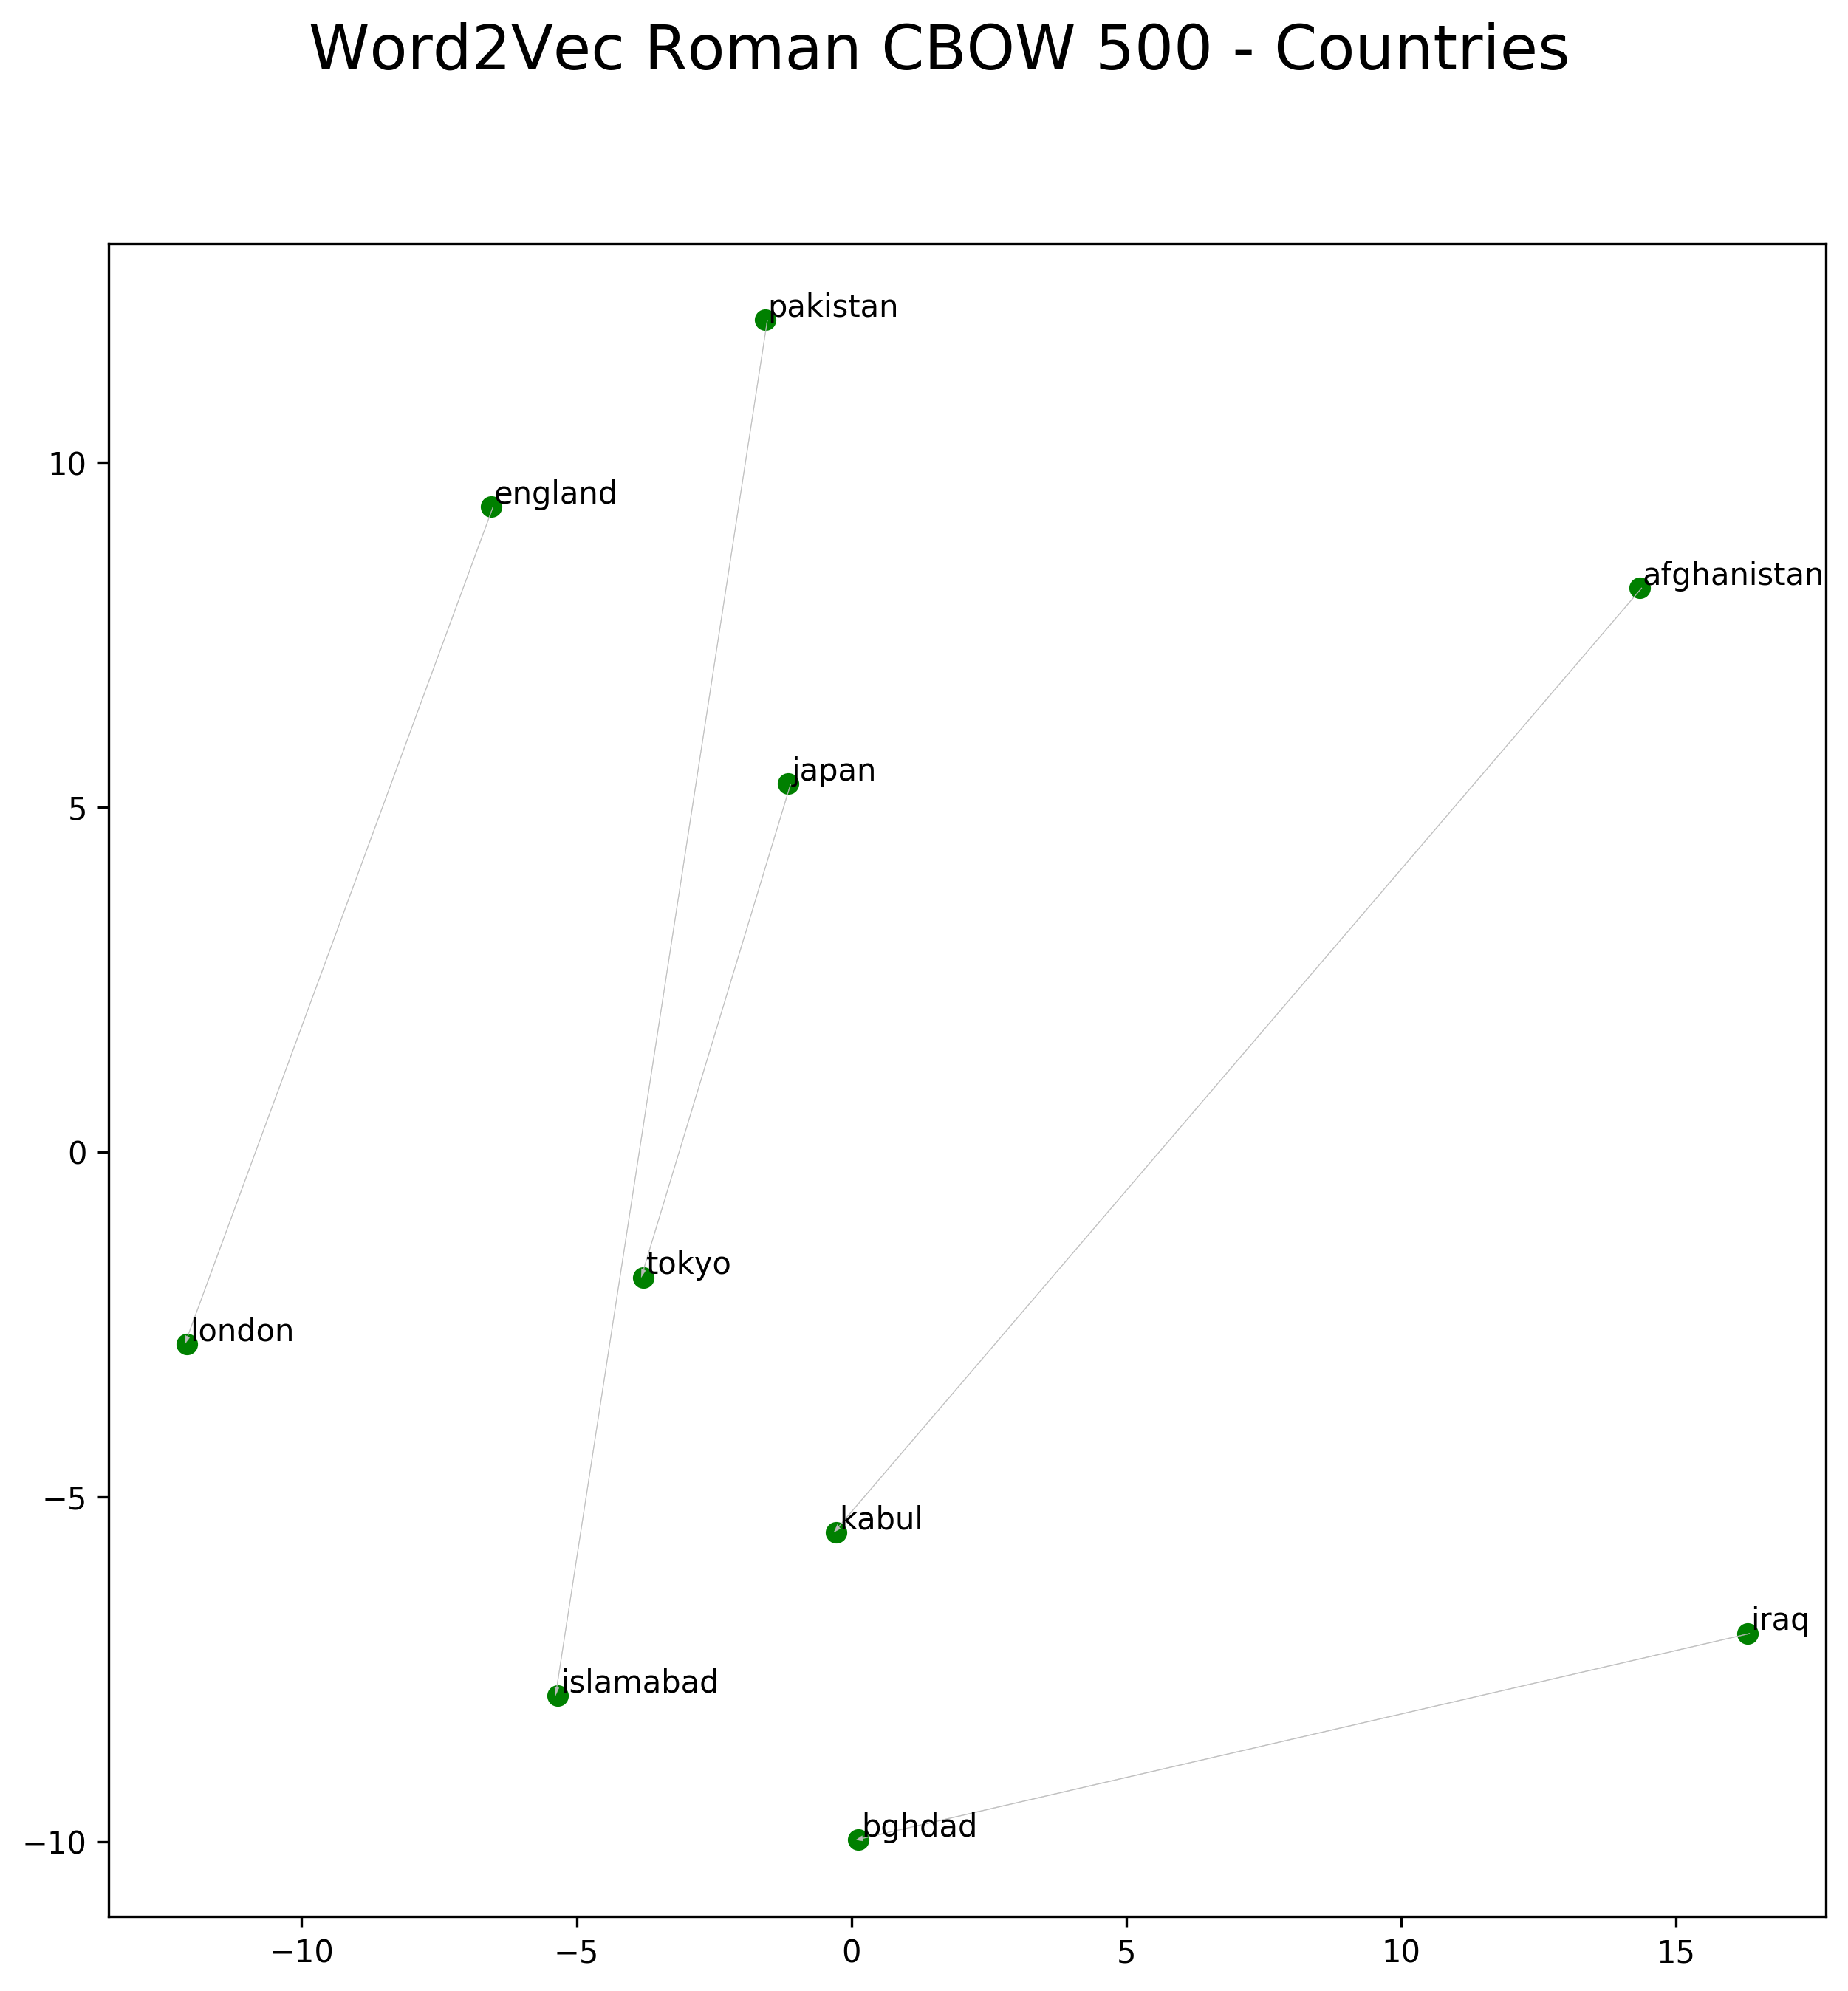
\includegraphics[width=10cm,height=10cm,keepaspectratio]{word2vec-cbow_roman-urdu_countries.png} \\
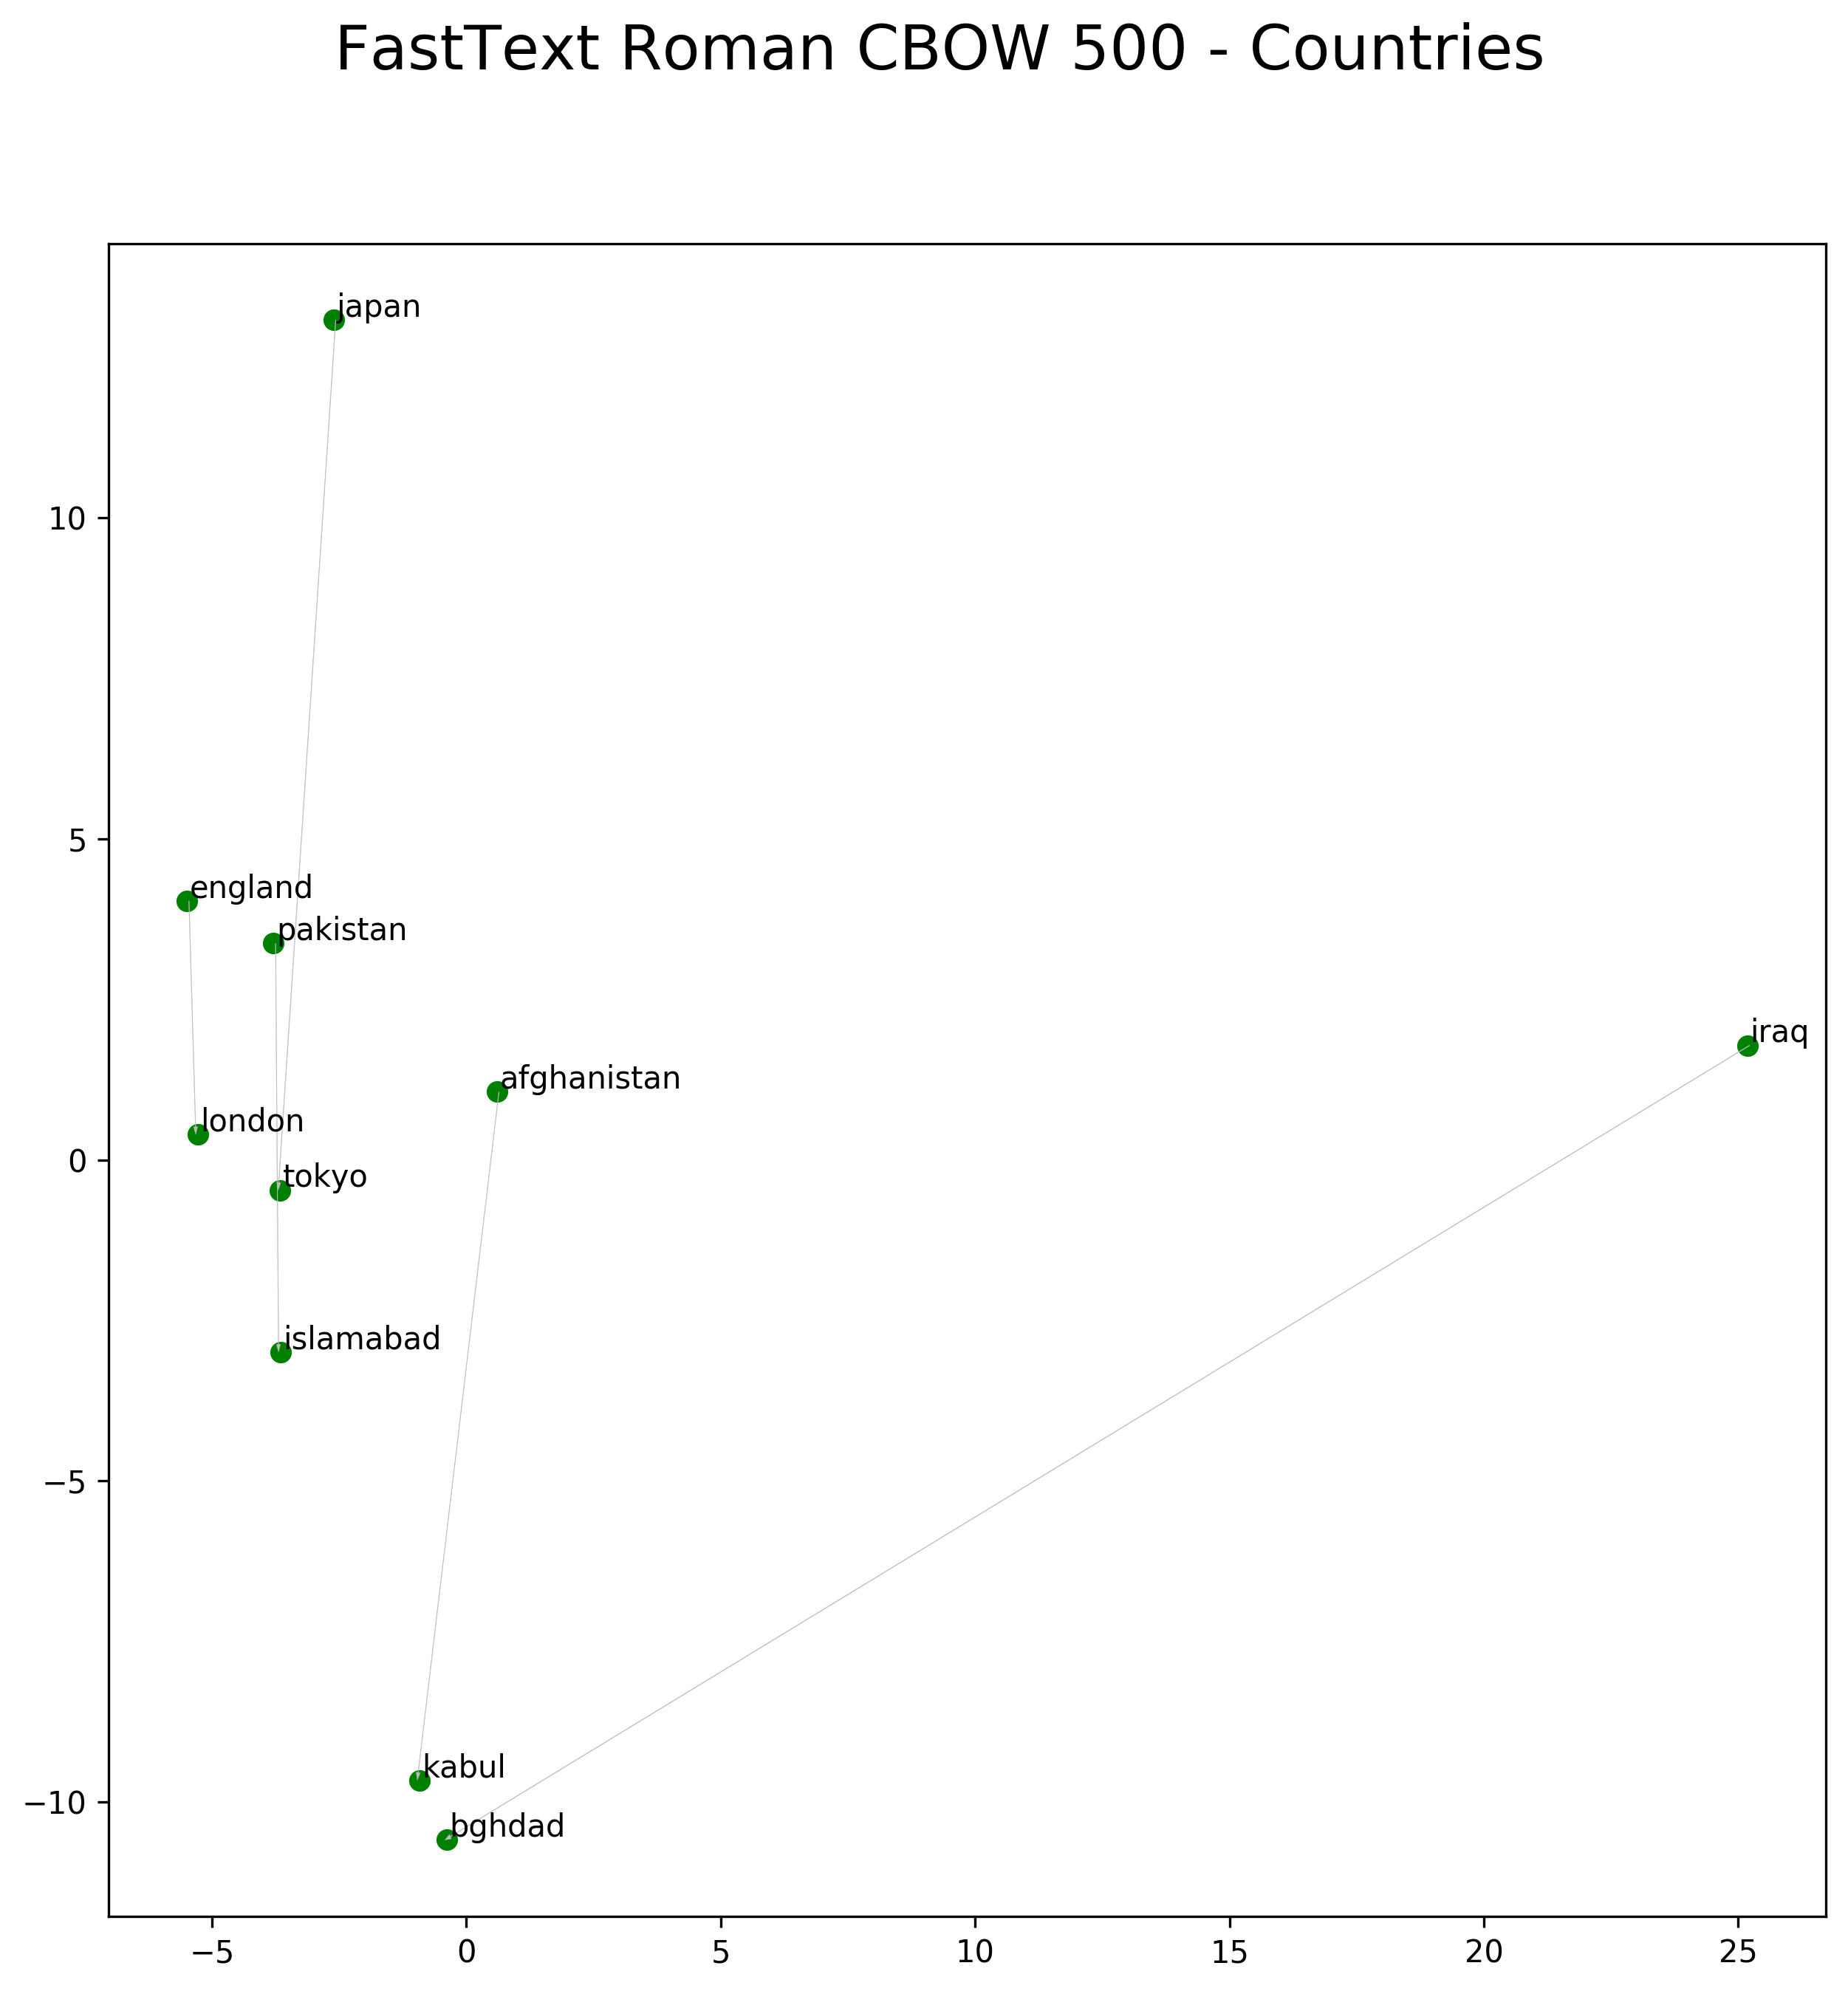
\includegraphics[width=10cm,height=10cm,keepaspectratio]{fasttext-cbow_roman-urdu_countries.png} \\


    \section{Conclusions and Future Work}
   We have successfully trained models of the Word2Vec, GloVe, fastText, ELMo and BERT techniques on our Urdu and Roman Urdu datasets and performed both qualitative and quantitative analyses. The main challenge we faced was the lack of publicly available, quality datasets for both the languages. These word embedding models can be evaluated using various NLP tasks like sentiment analysis, named entity recognition and part-of-speech classification, to name a few. However, each of these techniques requires the availability of a dataset designed for that specific task, in order to fine-tune a model for it. We could not find any such datasets for these languages. Due to this reason, we resorted to translating a couple of benchmark datasets namely: Wordsim-353 and Simlex-999 for a word similarity task to evaluate our models. This turned out to be problematic in our research when we attempted to use the same for evaluating BERT and ELMo, since they require a context to be provided to give meaningful word representations. Most evaluation methods and benchmarks described in \cite{devlin2018bert} and \cite{peters2018deep}  are exclusive to only a few high-resource languages and translating them for the sake of analysis was outside the scope of our project. We are able to find only one compatible benchmark, XNLI, for which we evaluated our BERT-Urdu model. \\
   
To advance research in the field of NLP for Urdu and Roman-Urdu, the biggest necessity is for quality datasets designed to perform various tasks as stated earlier. For future work, a more diverse and comprehensive dataset for Urdu and Roman Urdu languages could be developed for improved analysis and comparison. Popular benchmark tests could be translated or new datasets may be developed to enable further research into this area. Newer developed models such as ALBERT \cite{lan2019albert} and RoBERTa \cite{liu2019roberta} could also be evaluated in the future and analyzed using the same methodologies that we applied in this research. 
    \bibliographystyle{ACM-Reference-Format}
    \bibliography{citations}
\end{document}